\documentclass{standalone}
\usepackage{tikz}
\usetikzlibrary{arrows,decorations.markings,decorations.pathreplacing,calc,positioning}

\begin{document}%
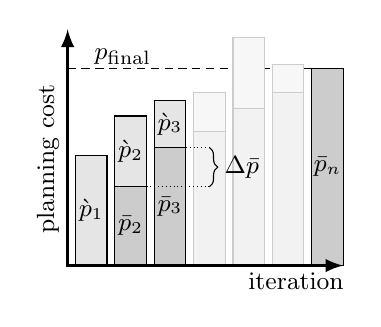
\begin{tikzpicture}[font=\small]

%\draw[black!5] (-0.1,-0.1) rectangle (3.6,3.6);
%\draw[step=0.5cm,black!20,very thin] (0,0) grid (3.5,3.5);

\draw[densely dashed] (0,2.5) -- (3.5,2.5);

% some bars
% col1
\draw[fill=black!10] (0.1,0) rectangle node[anchor=center]{$\grave{p}_1$} (0.5,1.4);

% col 2
\draw[fill=black!20] (0.6,0.0) rectangle node[anchor=center]{$\bar{p}_2$}   (1.0,1.0);
\draw[fill=black!10] (0.6,1.0) rectangle node[anchor=center]{$\grave{p}_2$} (1.0,1.9);

% col 3
\draw[fill=black!20] (1.1,0.0) rectangle node[anchor=center]{$\bar{p}_3$}   (1.5,1.5);
\draw[fill=black!10] (1.1,1.5) rectangle node[anchor=center]{$\grave{p}_3$} (1.5,2.1);

% col 4
\draw[black!20,fill=black!05] (1.6,0.0) rectangle node[anchor=center]{}   (2.0,1.7);
\draw[black!20,fill=black!03] (1.6,1.7) rectangle node[anchor=center]{} (2.0,2.2);

% col 5
\draw[black!20,fill=black!05] (2.1,0.0) rectangle node[anchor=center]{}   (2.5,2.0);
\draw[black!20,fill=black!03] (2.1,2.0) rectangle node[anchor=center]{} (2.5,2.9);

% col 6
\draw[black!20,fill=black!05] (2.6,0.0) rectangle node[anchor=center]{}   (3.0,2.2);
\draw[black!20,fill=black!03] (2.6,2.2) rectangle node[anchor=center]{} (3.0,2.55);

% col 7
\draw[black,fill=black!20] (3.1,0.0) rectangle node[black,anchor=center]{$\bar{p}_n$}   (3.5,2.5);

\draw[densely dotted] (1.0,1.0) -- (1.8,1.0);
\draw[densely dotted] (1.5,1.5) -- (1.8,1.5);
\draw [decorate,decoration={brace,amplitude=3pt,mirror},xshift=0pt,yshift=0pt]
(1.8,1.0) -- (1.8,1.5) node[anchor=west] [black,midway,xshift=2pt] 
{$\Delta\bar{p}$};

% axes
\draw[black,very thick,latex-latex] (0,3.0) -- (0,0) -- (3.5,0);

\node at (2.9,-0.2) {iteration};

\node[rotate=90] at (-0.25,1.35) {planning cost};

\node at (0.7,2.65) {$p_{\mbox{\scriptsize final}}$};

\end{tikzpicture}
\end{document}
